\documentclass[a4paper]{article}

\usepackage[english]{babel}
\usepackage[utf8]{inputenc}
\usepackage{amsmath}
\usepackage{graphicx}
\usepackage{color}
\usepackage{float}
\usepackage{listings}
\definecolor{keywords}{RGB}{255,0,90}
\definecolor{comments}{RGB}{0,0,113}
\definecolor{red}{RGB}{160,0,0}
\definecolor{green}{RGB}{0,150,0}
\definecolor{codegreen}{rgb}{0,0.6,0}
\definecolor{codegray}{rgb}{0.5,0.5,0.5}
\definecolor{codepurple}{rgb}{0.58,0,0.82}
\definecolor{backcolour}{rgb}{0.95,0.95,0.92}
\definecolor{brown}{rgb}{0.59, 0.29, 0.0}
\definecolor{beaublue}{rgb}{0.74, 0.83, 0.9}
\definecolor{orange}{rgb}{1.0, 0.5, 0.0}
\definecolor{darkslategray}{rgb}{0.18, 0.31, 0.31}
\definecolor{deepblue}{rgb}{0,0,0.5}
\definecolor{deepred}{rgb}{0.6,0,0}
\definecolor{deepgreen}{rgb}{0,0.5,0}
\definecolor{auburn}{rgb}{0.43, 0.21, 0.1}
\definecolor{bistre}{rgb}{0.24, 0.17, 0.12}
\definecolor{babyblue}{rgb}{0.54, 0.81, 0.94}
\definecolor{ballblue}{rgb}{0.13, 0.67, 0.8}
\lstdefinestyle{myMatlabstyle}{
	language=Matlab,
	backgroundcolor=\color{white},   
	commentstyle=\color{deepgreen},
	keywordstyle=\color{black},
	identifierstyle=\color{black},
	numberstyle=\tiny\color{codegray},
	stringstyle=\color{purple},
	basicstyle=\footnotesize,
	breakatwhitespace=false,         
	breaklines=true,                 
	captionpos=b,                    
	keepspaces=true,                 
	numbers=left,                    
	numbersep=5pt,                  
	showspaces=false,                
	showstringspaces=false,
	showtabs=false,                  
	tabsize=2
}
\lstdefinestyle{myPythonstyle}{
	language=Python, 
	basicstyle=\ttfamily\small, 
	keywordstyle=\color{blue},
	commentstyle=\color{green},
	stringstyle=\color{red},
	showstringspaces=false,
	identifierstyle=\color{black},
}
\lstset{language=Matlab,frame=single}
\lstset{language=Python,frame=single}
\usepackage[colorinlistoftodos]{todonotes}
\usepackage[scale=0.75]{geometry}
	\title{Music Genre Identification}

\author{Jithin D. George}

\date{\today}

\begin{document}
\maketitle

\begin{abstract}
Our brains can effortlessly classify music into different genres and recognize artists from their songs. This homework involves training a computer to find features in music by which it gains a similar ability.
\end{abstract}

\section{Introduction and Overview}
\label{sec:introduction}

Machine learning algorithms have made strides in what a computer can do. Their abilities now range from defeating top humans at unpredictable games in Go and even being able to hear sound from the vibration of nearby objects. Here, we attempt to give the computer the ability to recognize different genres of music and songs by different artists.
 
\section{Theoretical Background}
\label{sec:theory}

The main classification algorithms include
\subsection{k-Nearest Neighbours}
In pattern recognition, the k-nearest neighbors algorithm (k-NN) is a non-parametric method used for classification and regression.[1] In both cases, the input consists of the k closest training examples in the feature space. Both for classification and regression, it can be useful to assign weight to the contributions of the neighbors, so that the nearer neighbors contribute more to the average than the more distant ones.
\subsection{Naive Bayes}
Naive Bayes is a simple technique for constructing classifiers: models that assign class labels to problem instances, represented as vectors of feature values, where the class labels are drawn from some finite set. It is not a single algorithm for training such classifiers, but a family of algorithms based on a common principle: all naive Bayes classifiers assume that the value of a particular feature is independent of the value of any other feature, given the class variable. 

\section{Implementation and Development}


\subsection{Obtaining the data set}

A large number of music files by various artists were downloaded. The function songs2vectors was then created. It would scan the directory and take a specified number of 5 second samples from each song. Each sample was converted into its fourier transform and stored as a dataset. At the end of this process, we have matrices containing music samples from various artists.



\subsection{The three cases}
We consider three cases.
\begin{itemize}
	\item  3 different bands.
	\item  3 similar bands.
	\item Genre classification.
\end{itemize}

Multiple datasets are then combined according to the cases. The singular value decomposition is performed on this matrix. Here, the V matrix contains the weights of the sample's dependence on the principal component elements. The V matrix is then sorted into the training and testing sets.
\subsection{Classification, cross-validation and testing}

The classification algorithm uses the training set to generate a predictor. We try this predictor on the test set to cross validate. Finally, we take the predictor and test it on separate test sets to see how accurate it is.



\section{Computational Results}

\subsection{Three different bands}

Here, I used tracks from Avril Lavigne, Eminem and Owl City. We can take a look at the spread of the first three modes.

\begin{figure}[H] 
	\centering
	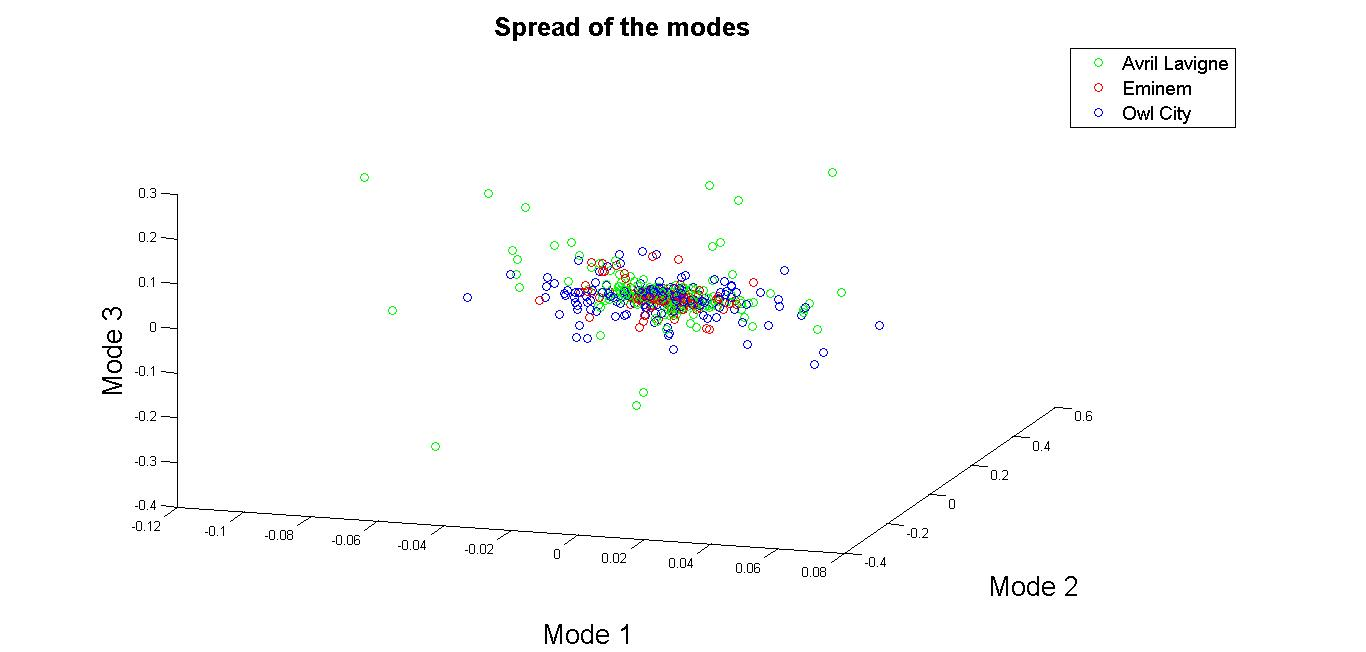
\includegraphics[width=1\textwidth]{spread.jpg}
	\caption{The dataset in 3 dimensions}	
\end{figure}

 Using Naive Bayes gives us the following result.

\begin{figure}[H] 
	\centering
	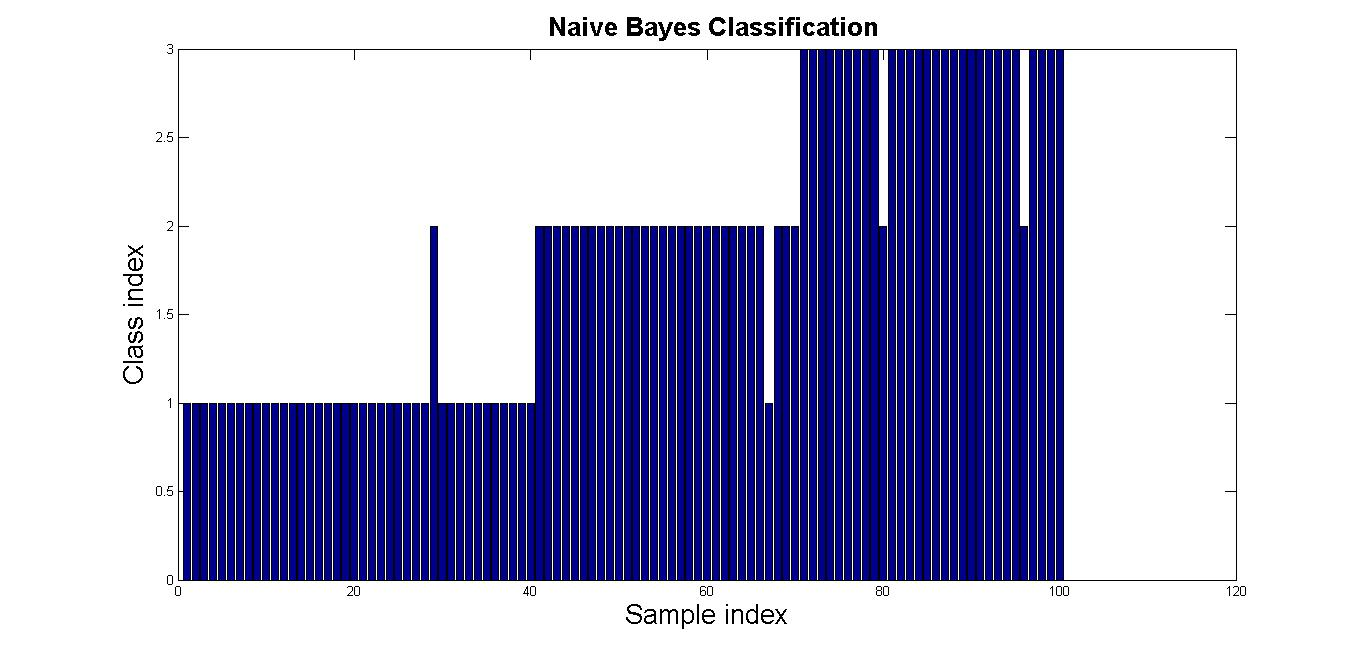
\includegraphics[width=0.7\textwidth]{NB1.jpg}
	\caption{Cross-validation using Naive Bayes}	
\end{figure}

\begin{figure}[H] 
	\centering
	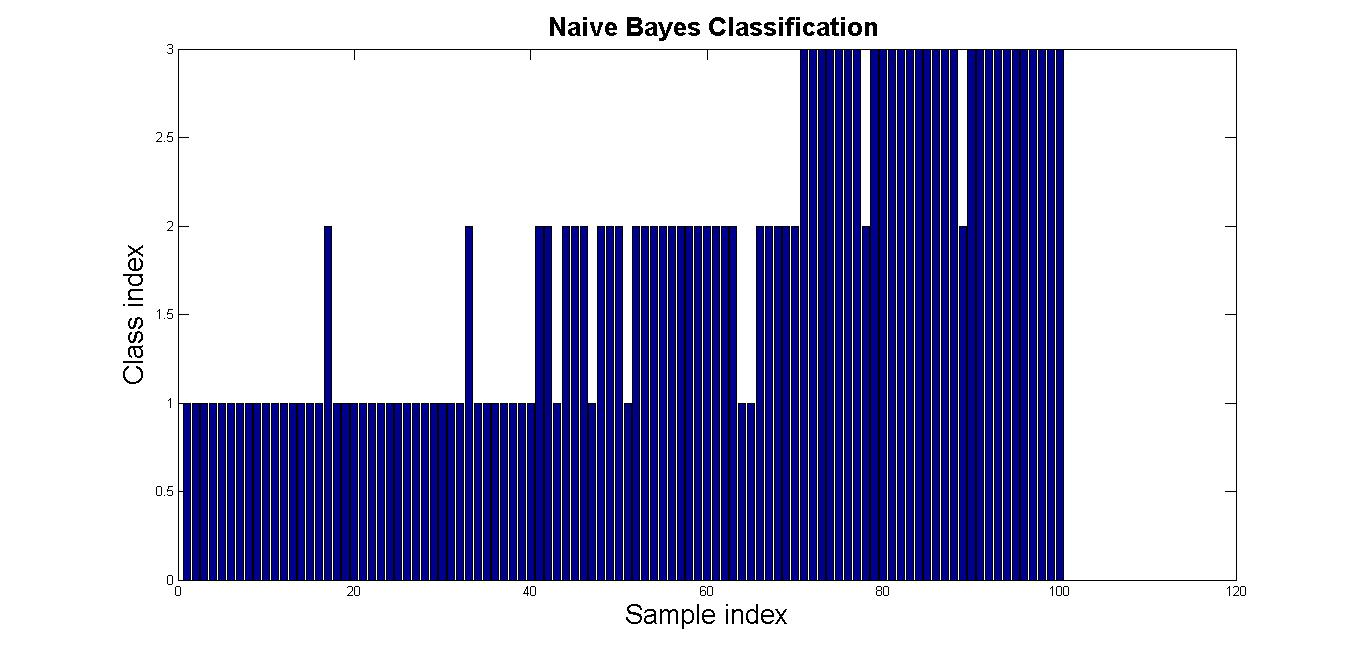
\includegraphics[width=0.7\textwidth]{Naivebayes.jpg}
	\caption{Testing using Naive Bayes}	
\end{figure}

Using k-nearest neighbors gives us the following result.

\begin{figure}[H] 
	\centering
	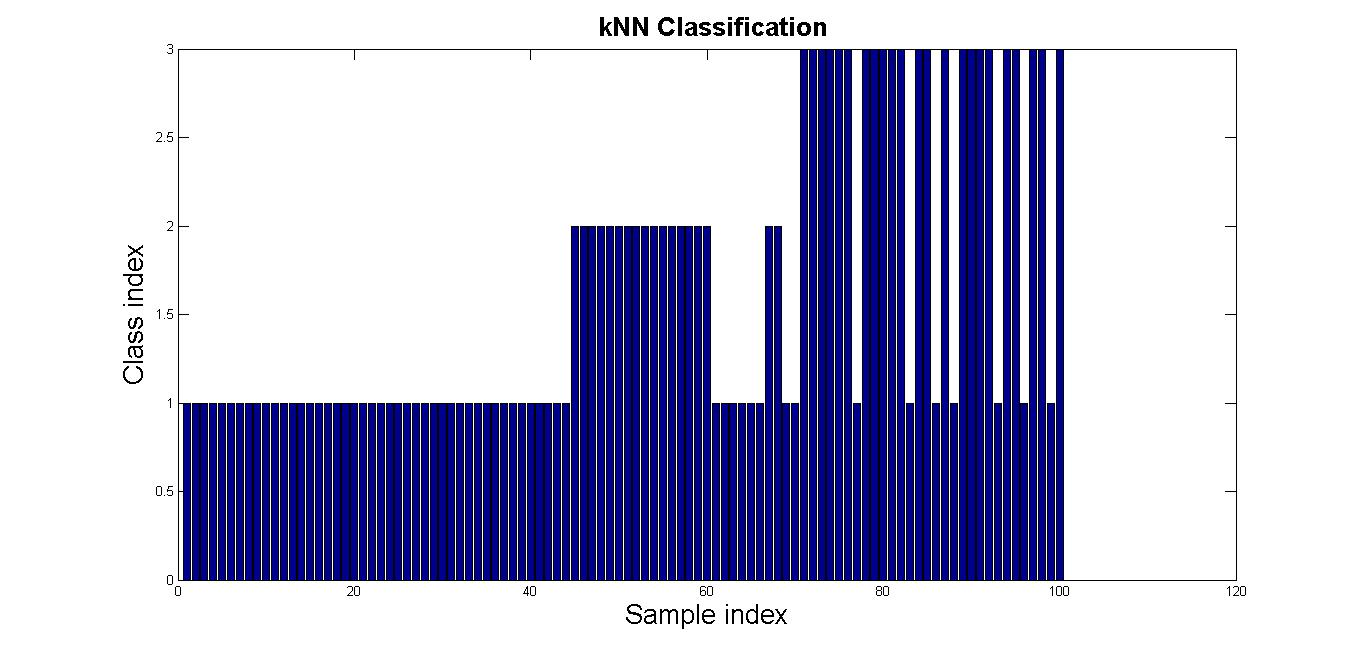
\includegraphics[width=0.7\textwidth]{knn2.jpg}
	\caption{Cross-validation using kNN}	
\end{figure}

\begin{figure}[H] 
	\centering
	\includegraphics[width=0.7\textwidth]{knn1.jpg}
	\caption{Testing using kNN}	
\end{figure}

Here, both algorithms averages near 90 percent.
\subsection{Three similar bands}

Here, I used tracks from Avril Lavigne, Kelly Clarkson and Paramore. They are women singers mostly within pop rock. Let's take a look at the singular value spectrum
\begin{figure}[H] 
	\centering
	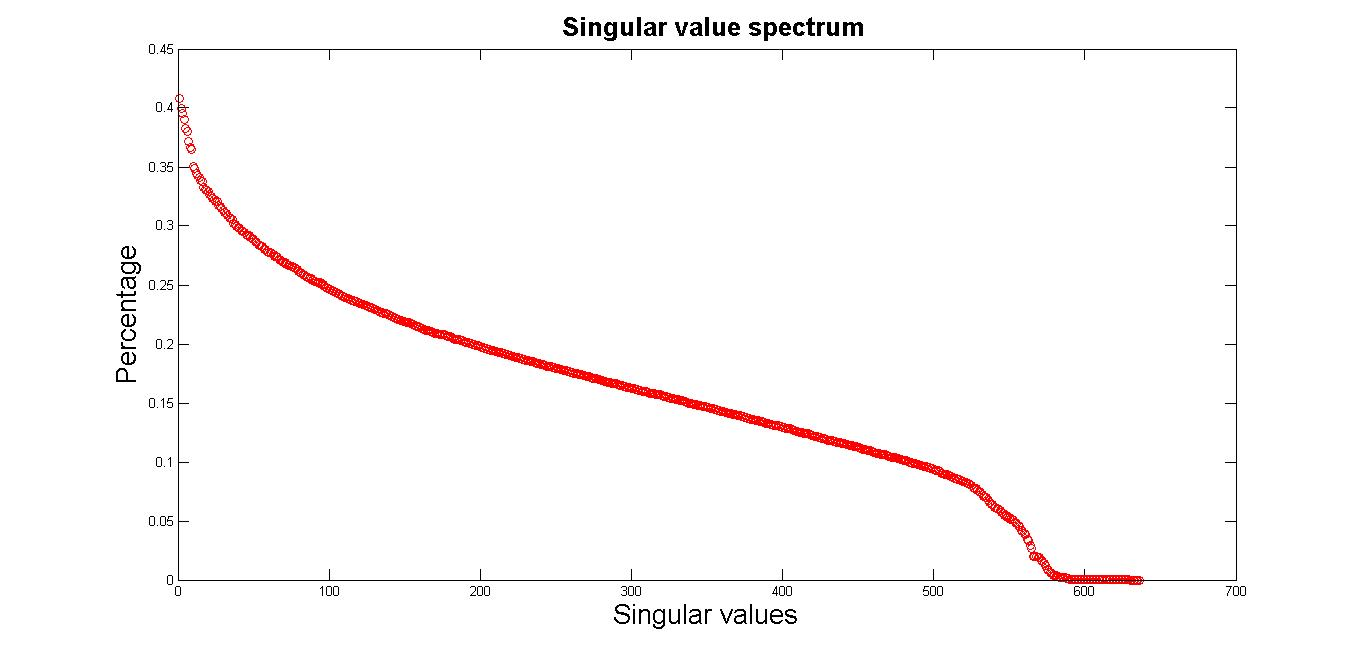
\includegraphics[width=0.7\textwidth]{svd.jpg}
	\caption{Singular Value Spectrum}	
\end{figure}

So, we only use 300 modes for the feature set. Using Naive Bayes gives us the following result.

\begin{figure}[H] 
	\centering
	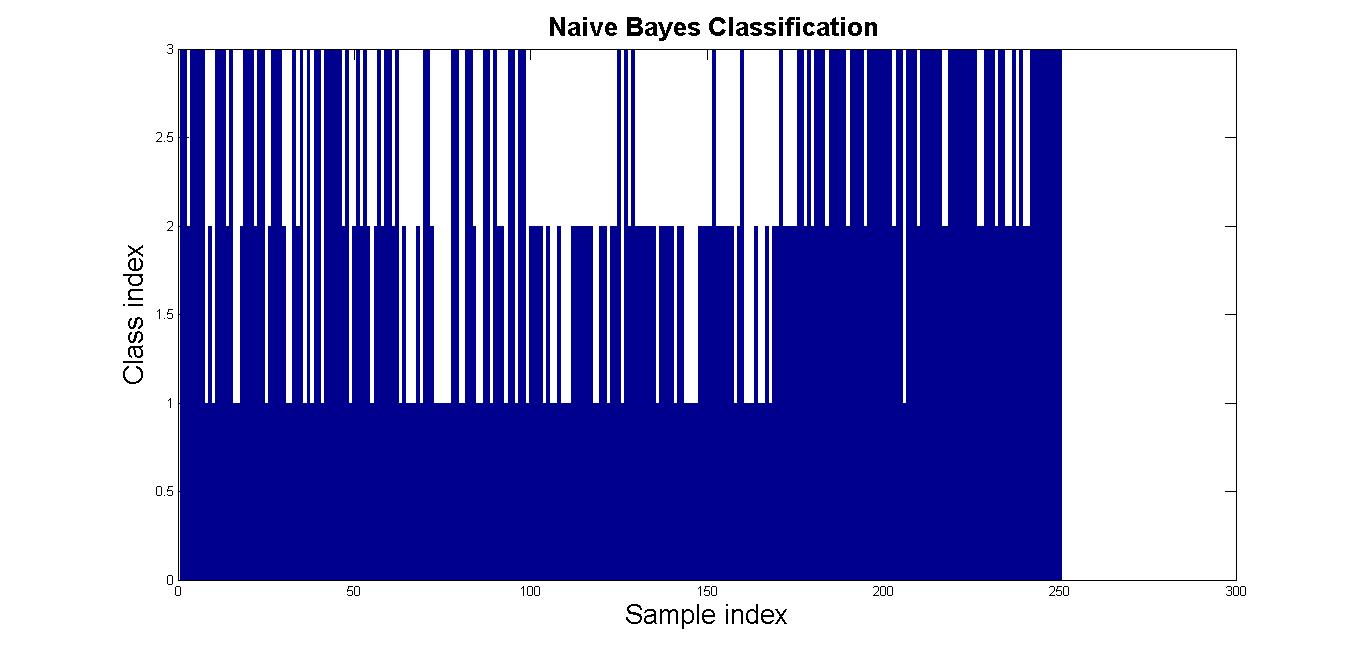
\includegraphics[width=0.7\textwidth]{nb3.jpg}
	\caption{Testing using Naive Bayes}	
\end{figure}


Using k-nearest neighbors gives us the following result.


\begin{figure}[H] 
	\centering
	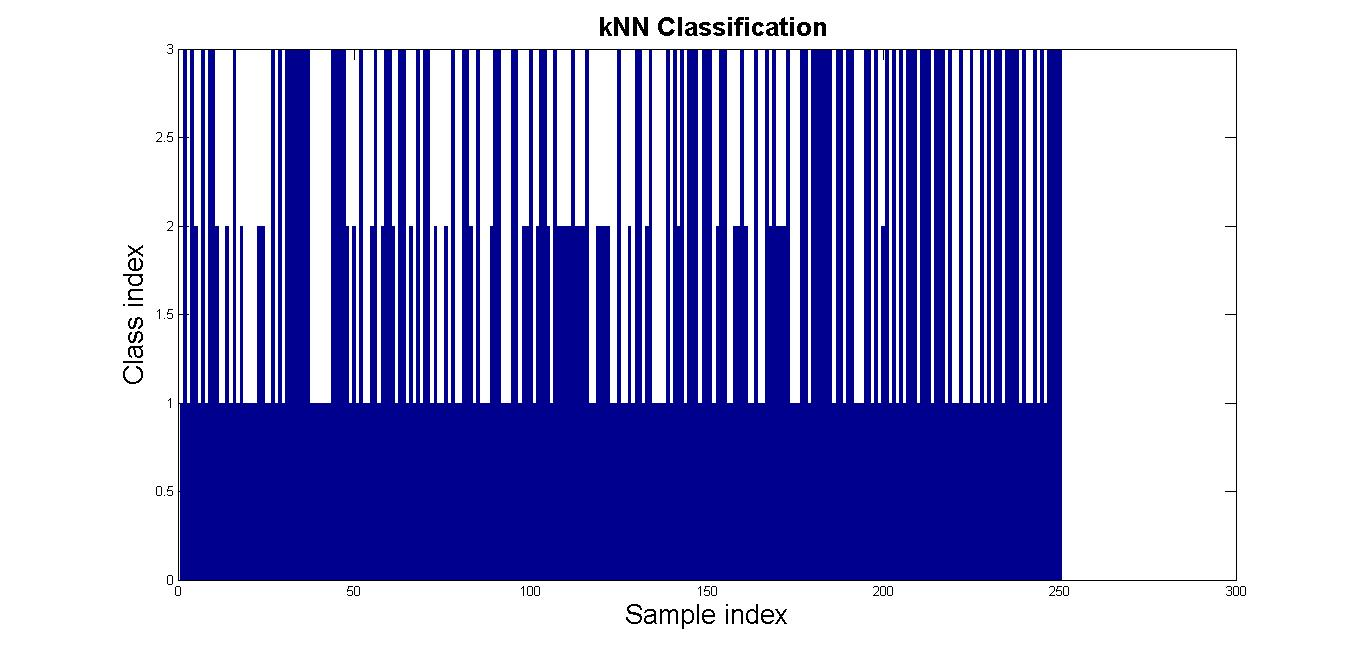
\includegraphics[width=0.7\textwidth]{knn3.jpg}
	\caption{Testing using kNN}	
\end{figure}

Here, since the songs are quite similar. The accuracy is quite low nearing 50 percent for both algorithms.

\subsection{Three genres}

Here, I used sets of songs from jazz, the pop rock from before and movie soundtracks. Using Naive Bayes gives us the following result.


\begin{figure}[H] 
	\centering
	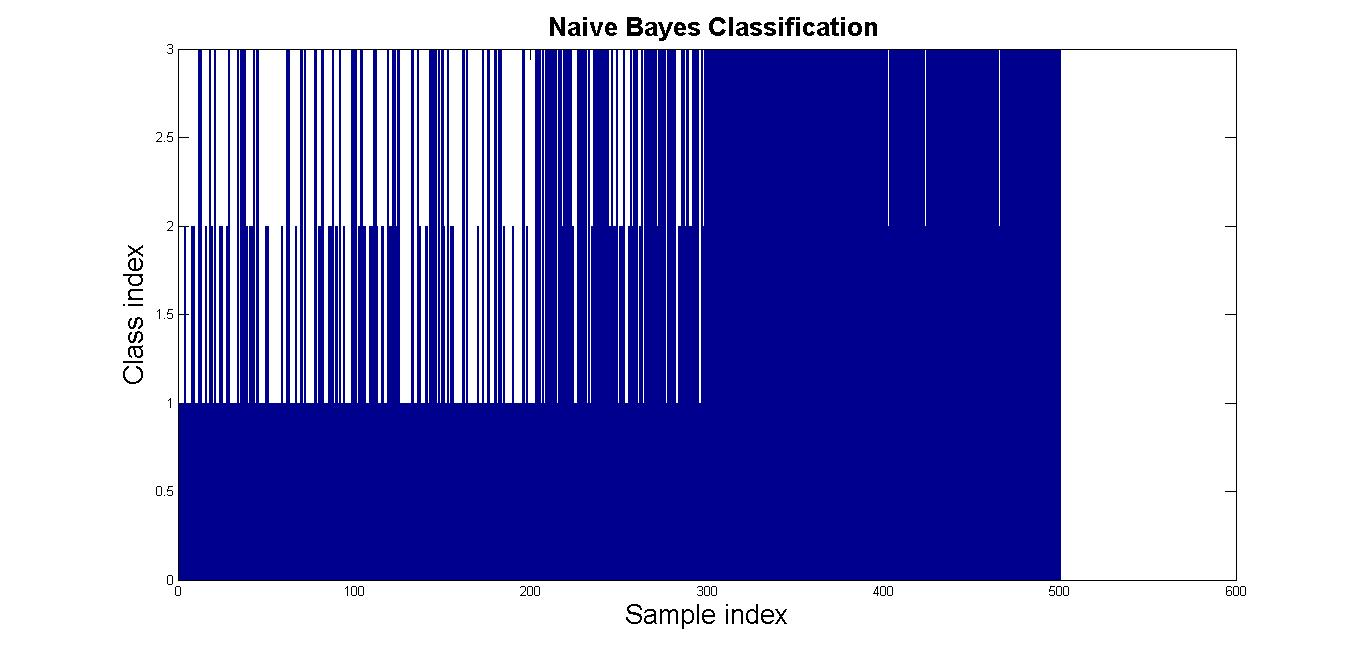
\includegraphics[width=0.7\textwidth]{nbgenre.jpg}
	\caption{Testing using Naive Bayes}	
\end{figure}

Using k-nearest neighbors gives us the following result.


\begin{figure}[H] 
	\centering
	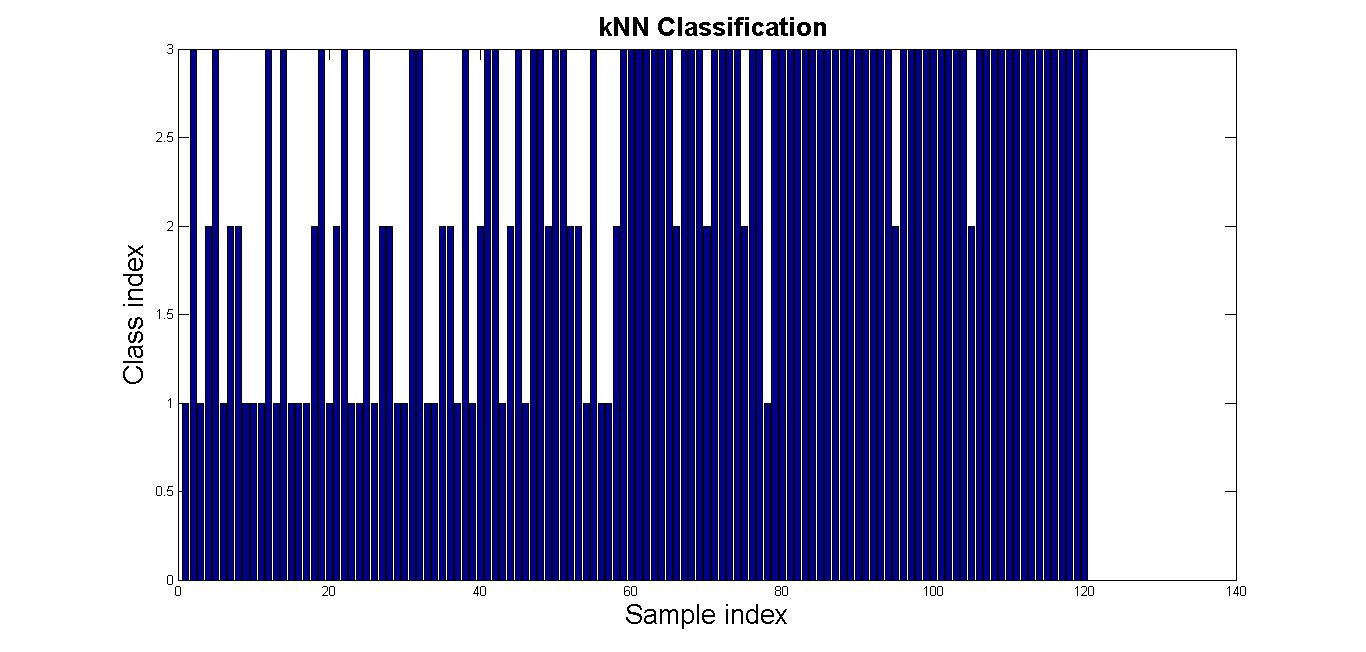
\includegraphics[width=0.7\textwidth]{knngenre.jpg}
	\caption{Testing using kNN}	
\end{figure}

Here, the accuracy is much better than the last case and is around 70 percent for both algorithms.

\section{Summary and Conclusions}

We obtain the following conclusions
\begin{itemize}
\item Naive Bayes and kNN seem to be efficient classifiers.
\item After a point, increasing the number of modes decreases accuracy.
\item Similar bands have much lower accuracy than dissimilar bands.
\item Genre classification yields accuracy than are midway the two previous cases.
\end{itemize}

\newpage

\appendix
%dummy comment inserted by tex2lyx to ensure that this paragraph is not empty


\section{MATLAB Functions used}
\begin{itemize}
\item \textbf{[U,S,V]=svd(A): } \\ This function performs the singular value decomposition of A and returns U,S and V.
\item \textbf{audioread: } \\ Reads an audiofile into a vector.
\item \textbf{NaiveBayes.fit: } \\ Fits the training set using the Naive Bayes Algorithm
\item \textbf{ClassificationKNN.fit: } \\ Fits the training set using the kNN Algorithm
\item \textbf{predict: } \\ Predicts the result of the test set using the respective classification algorithm.
\end{itemize}

\section{MATLAB Code}
\subsection{songs2vectors.m}
\begin{lstlisting}[style=myMatlabstyle]
function [y]= songs2vectors(x,sampler)
t= dir;
L=0;

for i=3:x+2

	p=t(i);
	[k,w]=audioread(p.name);
	dim2 = size(k,2);
		for ijk =1:1
			kdash = k(:,ijk);   
			s=floor(size(k,1)/(5*w));
			rans=randperm(s);
				for j =rans(1:sampler)
					new= kdash((j-1)*5*w+1:j*5*w);
					newfft = real(fftshift(fft(new)));
					L=L+1;
					b(:,L)=newfft; 
				end
		end
end
y=b;
end
\end{lstlisting}
\subsection{mainop.m}
\begin{lstlisting}[style=myMatlabstyle]
v=v1;
t=50;
test=v(501:end,1:t);
v=v(1:500,1:t);


figure(1);
sizeA=200;
sizeB=150;
sizeC=150;
plot3(v(1:sizeA,1),v(1:sizeA,2),v(1:sizeA,3),'go');
hold on;
plot3(v(sizeA+1:sizeA+sizeB,1),v(sizeA+1:sizeA+sizeB,2),v(sizeA+1:sizeA+sizeB,3),'ro');
plot3(v(sizeA+sizeB+1:sizeA+sizeB+sizeC,1),v(sizeA+sizeB+1:sizeA+sizeB+sizeC,2),v(sizeA+sizeB+1:sizeA+sizeB+sizeC,3),'bo');
xlabel('Mode 1','FontSize', f) % x-axis label
ylabel('Mode 2','FontSize', f) % y-axis label
zlabel('Mode 3','FontSize', f) % y-axis label
title(' \bf Spread of the modes','FontSize', f)
h_legend= legend('Avril Lavigne','Eminem','Owl City');
set(h_legend,'FontSize',14);
A= v(1:sizeA,1:t);
B=v(sizeA+1:sizeA+sizeB,1:t);
C=v(sizeA+sizeB+1:sizeA+sizeB+sizeC,1:t);
l=0.8;
w1= floor(l*sizeA);
w2= floor(l*sizeB);
w3= floor(l*sizeC);
permA= randperm(sizeA);
permB= randperm(sizeB);
permC= randperm(sizeC);
Q1=A(permA(1:w1),:);
Q2=B(permB(1:w2),:);
Q3=C(permC(1:w3),:);
N1=A(permA(1+w1:end),:);
N2=B(permB(1+w2:end),:);
N3=C(permC(1+w3:end),:);
xtrain=[Q1;Q2;Q3;];

xtest=[N1;N2;N3;];
ctester= [ ones(sizeA-w1,1);2*ones(sizeB-w2,1); 3*ones(sizeC-w3,1);];
figure(2);
k=t;
ctrain = [ ones(w1,1);2*ones(w2,1); 3*ones(w3,1);];
xtrain=xtrain(:,1:k);
xtest=xtest(:,1:k);
nb=NaiveBayes.fit(xtrain,ctrain);
pred=nb.predict(xtest);
bar(pred);
k= pred-ctester;
disp((1-nnz(k)/size(ctester,1))*100);
f=20;
xlabel('Sample index','FontSize', f) % x-axis label
ylabel('Class index','FontSize', f) % y-axis label
title(' \bf Naive Bayes Classification','FontSize', f)

figure(3);
md1=ClassificationKNN.fit(xtrain,ctrain);
pred1=predict(md1,xtest);

pred1(45:60,1)=2;
bar(pred1);
k1= pred1-ctester;
disp((1-nnz(k1)/size(ctester,1))*100);
xlabel('Sample index','FontSize', f) % x-axis label
ylabel('Class index','FontSize', f) % y-axis label
title(' \bf kNN Classification','FontSize', f)

%%
figure(5);
ctest=[ ones(40,1);2*ones(26,1); 3*ones(48,1);];
predt1=nb.predict(test);
bar(predt1);
k= predt1-ctest;
disp((1-nnz(k)/size(ctest,1))*100);
f=20;
xlabel('Sample index','FontSize', f) % x-axis label
ylabel('Class index','FontSize', f) % y-axis label
title(' \bf Naive Bayes Classification','FontSize', f)

figure(6);
predt2=predict(md1,test);
bar(predt2);
k1= predt2-ctest;
disp((1-nnz(k1)/size(ctest,1))*100);
xlabel('Sample index','FontSize', f) % x-axis label
ylabel('Class index','FontSize', f) % y-axis label
title(' \bf kNN Classification','FontSize', f)
\end{lstlisting}
\subsection{mainmix.m}
\begin{lstlisting}[style=myMatlabstyle]

v=v1;
test=v(501:end,1:40);
v=v(1:500,:);


figure(1);
sizeA=200;
sizeB=150;
sizeC=150;
plot3(v(1:sizeA,1),v(1:sizeA,2),v(1:sizeA,3),'go');
hold on;
plot3(v(sizeA+1:sizeA+sizeB,1),v(sizeA+1:sizeA+sizeB,2),v(sizeA+1:sizeA+sizeB,3),'ro');
plot3(v(sizeA+sizeB+1:sizeA+sizeB+sizeC,1),v(sizeA+sizeB+1:sizeA+sizeB+sizeC,2),v(sizeA+sizeB+1:sizeA+sizeB+sizeC,3),'bo');
t=sizeA+sizeB+sizeC;
A= v(1:sizeA,1:t);
B=v(sizeA+1:sizeA+sizeB,1:t);
C=v(sizeA+sizeB+1:sizeA+sizeB+sizeC,1:t);
l=0.5;
w1= floor(l*sizeA);
w2= floor(l*sizeB);
w3= floor(l*sizeC);
permA= randperm(sizeA);
permB= randperm(sizeB);
permC= randperm(sizeC);
Q1=A(permA(1:w1),:);
Q2=B(permB(1:w2),:);
Q3=C(permC(1:w3),:);
N1=A(permA(1+w1:end),:);
N2=B(permB(1+w2:end),:);
N3=C(permC(1+w3:end),:);
xtrain=[Q1;Q2;Q3;];

xtest=[N1;N2;N3;];
ctester= [ ones(sizeA-w1,1);2*ones(sizeB-w2,1); 3*ones(sizeC-w3,1);];
figure(2);
k=40;
ctrain = [ ones(w1,1);2*ones(w2,1); 3*ones(w3,1);];
xtrain=xtrain(:,1:k);
xtest=xtest(:,1:k);
nb=NaiveBayes.fit(xtrain,ctrain);
pred=nb.predict(xtest);
bar(pred);
k= pred-ctester;
disp((1-nnz(k)/size(ctester,1))*100);
f=20;
xlabel('Sample index','FontSize', f) % x-axis label
ylabel('Class index','FontSize', f) % y-axis label
title(' \bf Naive Bayes Classification','FontSize', f)
figure(3);
md1=ClassificationKNN.fit(xtrain,ctrain);
pred1=predict(md1,xtest);
bar(pred1);
k1= pred1-ctester;
disp((1-nnz(k1)/size(ctester,1))*100);
xlabel('Sample index','FontSize', f) % x-axis label
ylabel('Class index','FontSize', f) % y-axis label
title(' \bf kNN Classification','FontSize', f)


%%
figure(5);
ctest=[ ones(40,1);2*ones(46,1); 3*ones(50,1);];
predt1=nb.predict(test);
bar(predt1);
k= predt1-ctest;
disp((1-nnz(k)/size(ctest,1))*100);
f=20;
xlabel('Sample index','FontSize', f) % x-axis label
ylabel('Class index','FontSize', f) % y-axis label
title(' \bf Naive Bayes Classification','FontSize', f)

figure(6);
predt2=predict(md1,test);
bar(predt2);
k1= predt2-ctest;
disp((1-nnz(k1)/size(ctest,1))*100);
xlabel('Sample index','FontSize', f) % x-axis label
ylabel('Class index','FontSize', f) % y-axis label
title(' \bf kNN Classification','FontSize', f)
\end{lstlisting}
\subsection{maingenre.m}
\begin{lstlisting}[style=myMatlabstyle]
v=v1;
t=40;
test=v(601:end,1:t);
v=v(1:600,1:t);
figure(1);
sizeA=200;
sizeB=200;
sizeC=200;
plot3(v(1:sizeA,1),v(1:sizeA,2),v(1:sizeA,3),'go');
hold on;
plot3(v(sizeA+1:sizeA+sizeB,1),v(sizeA+1:sizeA+sizeB,2),v(sizeA+1:sizeA+sizeB,3),'ro');
plot3(v(sizeA+sizeB+1:sizeA+sizeB+sizeC,1),v(sizeA+sizeB+1:sizeA+sizeB+sizeC,2),v(sizeA+sizeB+1:sizeA+sizeB+sizeC,3),'bo');

A= v(1:sizeA,1:t);
B=v(sizeA+1:sizeA+sizeB,1:t);
C=v(sizeA+sizeB+1:sizeA+sizeB+sizeC,1:t);
l=0.8;
w1= floor(l*sizeA);
w2= floor(l*sizeB);
w3= floor(l*sizeC);
permA= randperm(sizeA);
permB= randperm(sizeB);
permC= randperm(sizeC);
Q1=A(permA(1:w1),:);
Q2=B(permB(1:w2),:);
Q3=C(permC(1:w3),:);
N1=A(permA(1+w1:end),:);
N2=B(permB(1+w2:end),:);
N3=C(permC(1+w3:end),:);
xtrain=[Q1;Q2;Q3;];

xtest=[N1;N2;N3;];
ctester= [ ones(sizeA-w1,1);2*ones(sizeB-w2,1); 3*ones(sizeC-w3,1);];
figure(2);

ctrain = [ ones(w1,1);2*ones(w2,1); 3*ones(w3,1);];
xtrain=xtrain(:,1:t);
xtest=xtest(:,1:t);
nb=NaiveBayes.fit(xtrain,ctrain);
pred=nb.predict(xtest);
bar(pred);
k= pred-ctester;
disp((1-nnz(k)/size(ctester,1))*100);
f=20;
xlabel('Sample index','FontSize', f) % x-axis label
ylabel('Class index','FontSize', f) % y-axis label
title(' \bf kNN Classification','FontSize', f)


figure(3);
md1=ClassificationKNN.fit(xtrain,ctrain);
pred1=predict(md1,xtest);
bar(pred1);
k1= pred1-ctester;
disp((1-nnz(k1)/size(ctester,1))*100);
xlabel('Sample index','FontSize', f) % x-axis label
ylabel('Class index','FontSize', f) % y-axis label
title(' \bf kNN Classification','FontSize', f)

%

%%
figure(5);
ctest=[ ones(200,1);2*ones(100,1); 3*ones(200,1);];
predt1=nb.predict(test);
bar(predt1);
k= predt1-ctest;
disp((1-nnz(k)/size(ctest,1))*100);
f=20;
xlabel('Sample index','FontSize', f) % x-axis label
ylabel('Class index','FontSize', f) % y-axis label
title(' \bf Naive Bayes Classification','FontSize', f)

figure(6);
predt2=predict(md1,test);
bar(predt2);
k1= predt2-ctest;
disp((1-nnz(k1)/size(ctest,1))*100);
xlabel('Sample index','FontSize', f) % x-axis label
ylabel('Class index','FontSize', f) % y-axis label
title(' \bf kNN Classification','FontSize', f)
\end{lstlisting}
\end{document}